% new_document_template.tex
% Clean starting point for school documents

\documentclass[a4paper,11pt]{article}
\usepackage{school-macros}
\usepackage[utf8]{inputenc}
\usepackage[dutch]{babel}
\usepackage{siunitx}
\usepackage{pdfpages}
\usepackage{float}
\usepackage{placeins}

% Add angles library for TikZ angle pictures
\usetikzlibrary{angles}


\title{Wisselstroom - Formularium met uitleg}
\author{Ruben Ryckaert}
\date{\today}

\begin{document}
\microtypecontext{spacing=nonfrench}
\maketitle
\tableofcontents
\printformularium
\newpage

\section{Inleiding}

In dit document wil ik alle belangrijke formules die je moet kennen geven.
Daarnaast geef ik ook een korte uitleg bij elke formule zodat je beter begrijpt wat er gebeurt.
Dit vak heeft nammelijk geen formularium op het examen
dus je moet deze allemaal goed kennen!

\section{Hoofdstuk 1: Basis wisselstroom theorie}

\frm{Wet van Ohm}{V = I \cdot R}{Met V de spanning in Volt, I de stroom in Ampère en R de weerstand in Ohm.}

\frm{$I(t)$}{I(t) = I_m \sin(\omega t)}{Met $I(t)$ de wisselstroom op tijdstip t, $I_m$ de piekstroom 
(maximale stroom) en $\omega$ de hoeksnelheid in rad/s.}

\frm{$V(t)$}{V(t) = V_m \sin(\omega t)}{Met $V(t)$ de wisselspanning op tijdstip t, $V_m$ de piekspannin
g (maximale spanning) en $\omega$ de hoeksnelheid in rad/s.}

\frm{$A_{gem}$}{A_{gem} = \frac{1}{T/2} \int_0^{T/2} A(t) dt}{Met $A_{gem}$ de gemiddelde waarde van A(t) 
over een halve periode T. Dit is handig voor wisselspanningen en -stromen omdat ze gemiddeld gezien 
0 zijn over een hele periode. De gemiddelde waarde geeft een beter idee van de effectieve grootte van de wisselstroom.}



met $a(t) = A_m \sin(\omega t)$
\[A_{gem} = \frac{1}{T/2} \int_0^{T/2} A_m \sin(\omega t) dt = \frac{2 A_m}{T} \left[ -\frac{1}{\omega} \cos(\omega t)
\right]_0^{T/2} = \frac{2 A_m}{T} \cdot \frac{2}{\omega} = \frac{2 A_m}{2\pi / \omega} \cdot \frac{2}{\omega} = \frac{2 A_m}{\pi}\]
\[A_{gem} = \frac{2 A_m}{\pi} = 0.64A_m\]


\frm{$A_{rms}$}{A_{rms} = \sqrt{\frac{1}{T} \int_0^T A^2(t) dt}}{Met $A_{rms}$ de effectieve waarde van A(t).
Dit is de waarde die je zou meten met een multimeter.}

met $a(t) = A_m \sin(\omega t)$
\[A_{rms} = \sqrt{\frac{1}{T} \int_0^T A_m^2 \sin^2(\omega t) dt} = A_m \sqrt{\frac{1}{T} \int_0^T \sin^2(\omega t) dt}
\]
\[= A_m \sqrt{\frac{1}{T} \cdot \frac{T}{2}} = A_m \cdot \frac{1}{\sqrt{2}} = 0.707 A_m\]

\vspace{0.3cm}

\subsection{fasors}

Een wisselstroom of -spanning kan je ook voorstellen als een roterende vector in het complexe vlak.
Dit noemen we een fasor.

\vspace{0.5cm}

\begin{figure}[H]
\centering
\begin{tikzpicture}[scale=1.5]
    % Assen tekenen
    \draw[->, thick] (-3,0) -- (3,0) node[right] {Re};
    \draw[->, thick] (0,-3) -- (0,3) node[above] {Im};
    
    % Grid lijnen
    \draw[gray!30, thin] (-2.5,-2.5) grid (2.5,2.5);
    
    % Fasor vector (bijvoorbeeld 45 graden)
    \draw[->, very thick, blue] (0,0) -- (2,2);
    
    % Hoek tonen
    \draw[red, thick] (0,0) -- (1.5,0) arc (0:45:1.5);
    \node[red] at (1.0,0.5) {$\phi$};
    
    % Projecties
    \draw[dashed, blue!60] (2,2) -- (2,0) node[below, yshift=-0.2cm] {$V \cos\phi$};
    \draw[dashed, blue!60] (2,2) -- (0,2) node[left, xshift=-0.2cm] {$V \sin\phi$};
    
    % Labels - positioned away from the vector
    \node[blue] at (2.3,2.3) {$V_m \angle \phi$};
    \node[blue] at (2.2,1.8) {$\vec{V}$};
\end{tikzpicture}
\caption{Weergave van een fasor in het complexe vlak. De fasor $\vec{V}$ heeft een amplitude $V_m$ en een fasehoek $\phi$. Het reële deel is $V \cos\phi$ en het imaginaire deel is $V \sin\phi$.}
\label{fig:fasor}
\end{figure}

Bij een fasor gaan we de hoeksnelheid $\omega$ niet meer expliciet noteren.
Als je een oefening voor het omzetten van fasor naar tijdsfunctie of omgekeerd doet,
ga je de hoeksnelheid gegeven krijgen.

\frm{fasor}{\vec{A} = A_m \angle \phi = A_m (\cos\phi + j \sin\phi) =A_m e^{j\phi}}{Met $\vec{A}$ de fasor van de wisselgrootte A,
$A_m$ de amplitude (piekwaarde) en $\phi$ de fasehoek in radialen. Het reële deel is $A_m \cos\phi$ 
en het imaginaire deel is $A_m \sin\phi$. }

\[A_m = \sqrt{(\text{Re}(\vec{A}))^2 + (\text{Im}(\vec{A}))^2}\]
\[\phi = \tan^{-1}\left(\frac{\text{Im}(\vec{A})}{\text{Re}(\vec{A})}\right)\]


voorbeeld: Alle notaties voor de functie $$v(t) = 220 \sin(314t + 30^\circ)$$

\[V_m = 220 V\]
\[\omega = 314 \text{ rad/s}\]
\[\phi = 30^\circ = \frac{\pi}{6} \text{ rad}\]

\[a = 220V \cdot \cos(30^\circ) = 190.5 V\]
\[b = 220V \cdot \sin(30^\circ) = 110 V\]
\[\vec{V} = 220 \angle 30^\circ = 220 (\cos 30^\circ + j \sin 30^\circ) =
 220 \left(\frac{\sqrt{3}}{2} + j \cdot \frac{1}{2}\right) = 190.5 + j 110 V\]

\section{Hoofdstuk 2: Wisselstroom ketens}

ELI the ICE man; L is de spoel, C is de condensator, I is de stroom, E is de spanning. Je kunt doen zien afhankelijk van 
welke weerstand of de stroom leading of lagging is.Als de stroom voorloopt op de spanning spreken we van een \textbf{leading} stroom.
Als de stroom achterloopt op de spanning spreken we van een \textbf{lagging} stroom.

\frm{Impedantie}{Z = R + jX}{Met Z de impedantie in Ohm, R de weerstand in Ohm en X de reactantie in Ohm.}

\frm{Reactantie spoel}{X_L = \omega L}{Met $X_L$ de inductieve reactantie in Ohm, $\omega$ de hoeksnelheid in rad/s en L de inductantie in Henry.}
\frm{Reactantie condensator}{X_C = \frac{-1}{\omega C}}{Met $X_C$ de capacatieve reactantie in Ohm, $\omega$ de hoeksnelheid in rad/s en C de capaciteit in Farad.}

\frm{Totale impedantie in serie}{Z_{totaal} = \sqrt{R^2 + (X_L + X_C)^2}}{Met $Z_{totaal}$ de totale impedantie in Ohm, R de weerstand in Ohm, $X_L$ de inductieve reactantie in Ohm en $X_C$ de capacatieve reactantie in Ohm.}

\frm{Hoek van de impedantie}{\tan \phi = \frac{X_L + X_C}{R}}{Met $\phi$ de fasehoek van de impedantie in radialen, R de weerstand in Ohm, $X_L$ de inductieve reactantie in Ohm en $X_C$ de capacatieve reactantie in Ohm.}


\subsection{Vermogen in wisselstroomkringen}
Door dat de stroom en voltage occeleren in tijd, gaat
het vermogen ook occeleren in tijd.

\begin{figure}[ht]
      \centering
        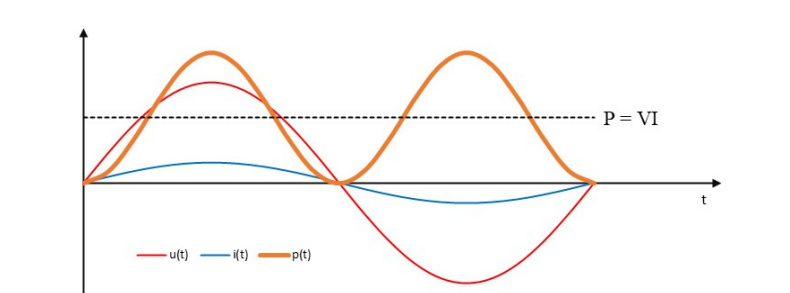
\includegraphics[width=0.8\textwidth]{vermogen.png}
        \caption{Vermogen in functie van tijd.}
        \label{fig:vermogen.png}
\end{figure}

\[p(t) = v(t) \cdot i(t) = V_m \sin(\omega t ) \cdot I_m \sin(\omega t)\]
\[= V_m I_m \sin^2(\omega t)\]
\[\sin^2(x) = \frac{1 - \cos(2x)}{2}\] (uit de goniometrische formules)
\[p(t) = V_m I_m \cdot \frac{1 - \cos(2\omega t)}{2} = \frac{V_m I_m}{2} (1 - \cos(2\omega t))\]
\[p(t) = V_m I_m \cdot \frac{1 - \cos(2\omega t)}{2} = \frac{V_m I_m}{2} (1 - \cos(2\omega t))\]

$$V_m I_m$$/2 zijn de rms waarde van spanning en stroom.

\[V_{rms} = \frac{V_m}{\sqrt{2}}\]
\[I_{rms} = \frac{I_m}{\sqrt{2}}\]
\[V_m I_m = \left(\frac{\sqrt{2}}{2} V_{rms}\right)\left(\frac{\sqrt{2}}{2} I_{rms}\right) = \left(\frac{\sqrt{2}}{2}\right)^2 V_{rms} I_{rms} = \frac{2}{4} V_{rms} I_{rms} = \frac{1}{2} V_{rms} I_{rms}\]


Afhankelijk van het circuit kan het zijn dat de stroom voorloopt of achterloopt op de spanning.

\begin{figure}[ht]
  \centering
      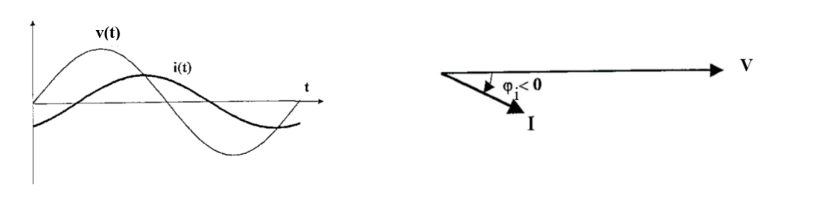
\includegraphics[width=0.8\textwidth]{stroomachtervoltage.png}
        \caption{Stroom die achterloopt op de spanning.} 
        \label{fig:stroomachtervoltage.png}
    \end{figure}

Welk vermogen wordt er nu verbruikt in het circuit?

\frm{Actief vermogen}{P = V_{rms} I_{rms} \cos \phi}{Met P het actieve vermogen in Watt, $V_{rms}$ de effectieve spanning in Volt, $I_{rms}$ de effectieve stroom in
 Ampère en $\phi$ de fasehoek tussen spanning en stroom in radialen.}

\frm{Schijnbaar vermogen}{S = V_{rms} I_{rms}}{Met S het schijnbaar vermogen in Volt-Ampère (VA), $V_{rms}$ 
de effectieve spanning in Volt en $I_{rms}$ de effectieve stroom in Ampère.}

\frm{reactief vermogen}{Q = V_{rms} I_{rms} \sin \phi}{Met Q het reactief vermogen in Volt-Ampère reactief (VAR), $V_{rms}$ 
de effectieve spanning in Volt, $I_{rms}$ de effectieve stroom in Ampère en $\phi$ de fasehoek tussen spanning en stroom in radialen.}

\begin{figure}[ht]
  \centering
      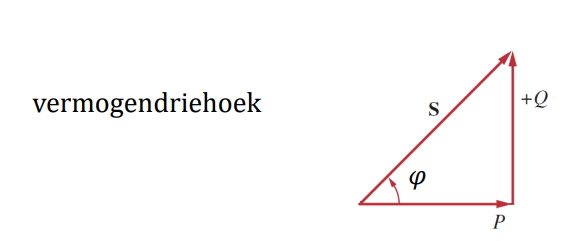
\includegraphics[width=0.6\textwidth]{Vermogendriehoek.png}
      \caption{Vermogendriehoek die de relatie toont tussen actief vermogen P, reactief vermogen Q en schijnbaar vermogen S.}
      \label{fig:Vermogendriehoek.png}
\end{figure}

\frm{Vermogendriehoek}{S = P + iQ}{Met S het schijnbaar vermogen in Volt-Ampère (VA), P het actieve vermogen 
in Watt en Q het reactief vermogen in Volt-Ampère reactief (VAR).}

\frm{Arbeidsfactor}{\text{arbeidsfactor} = \cos \phi = \frac{P}{S}}{Met de arbeidsfactor de verhouding is tussen het actieve vermogen P en het 
schijnbaar vermogen S. Het geeft aan welk deel van het schijnbaar vermogen daadwerkelijk wordt omgezet in nuttig werk.}

Laten we een voorbeeld bekijken:

$$V = 110\angle 85^\circ,\ I = 0.4\angle 15^\circ$$
Wat is de $a)$ het schijnbaar vermogen, $b)$ het actieve vermogen, $c)$ het reactief vermogen en $d)$ de arbeidsfactor en impedantie?

\[S = V_{rms} I_{rms} = 110 \cdot 0.4 = 44\ \mathrm{VA} \]
\[P = V_{rms} I_{rms} \cos \phi = 110 \cdot 0.4 \cdot \cos(85^\circ - 15^\circ) = 44 \cdot \cos 70^\circ = 15.05\ \mathrm{W}\]
\[Q = V_{rms} I_{rms} \sin \phi = 110 \cdot 0.4 \cdot \sin(85^\circ - 15^\circ) = 44 \cdot \sin 70^\circ = 41.36\ \mathrm{VAR} \]
\[\text{arbeidsfactor} = \cos \phi = \frac{P}{S} = \frac{15.05}{44} = 0.342\]
Positief dus de stroom loopt achter op de spanning.
\[\boxed{Z = \frac{V}{I} = \frac{110\angle 85^\circ}{0.4\angle 15^\circ} = 275\angle 70^\circ\ \Omega = 94 + j258.8\ \Omega}\]

\begin{examenbox}
Zorg dat je goed deze fasordiagrammen begrijpt. 
Je kunt echt een hele oefening oplossen door je fasors deftig te tekenen.
Weet dat imaginaire impedanties (zoals spoelen en condensatoren) 90 graden verschoven zijn tov reële impedanties (zoals weerstanden).
\end{examenbox}

Als je goed je fasors definieerd kun je geometrische formules gebruiken 
om uitkomsten te berekenen.

\frm{cosine regel}{c^2 = a^2 + b^2 - 2ab \cos \theta}{Met a, b en c de lengtes van de zijden van een driehoek 
en $\theta$ de hoek tegenover zijde c.}
\frm{sine regel}{\frac{a}{\sin A} = \frac{b}{\sin B} = \frac{c}{\sin C}}{Met a, b en c de lengtes van de zijden van een driehoek
  en A, B en C de hoeken tegenover zijden a, b en c respectievelijk.}

\vspace{0.5cm}

\begin{figure}[H]
\centering
\begin{tikzpicture}[scale=1.6, line cap=round, line join=round]
  % Vertices (scalene triangle)
  \coordinate (A) at (0,0);
  \coordinate (B) at (4.0,0);
  \coordinate (C) at (1.3,2.4);

  % Triangle
  \draw[thick] (A) -- (B) -- (C) -- cycle;
  \fill (A) circle (0.03);
  \fill (B) circle (0.03);
  \fill (C) circle (0.03);

  % Vertex labels
  \node[red, font=\small, below left]  at (A) {$A$};
  \node[red, font=\small, below right] at (B) {$B$};
  \node[red, font=\small, above]      at (C) {$C$};

  % Side labels (a opposite A, b opposite B, c opposite C)
  \path (B) -- (C) node[midway, right,  font=\small, text=blue] {$a$};
  \path (A) -- (C) node[midway, left,   font=\small, text=blue] {$b$};
  \path (A) -- (B) node[midway, below,  font=\small, text=blue] {$c$};

  % Angle marker at C (theta)
  \pic[draw=red, angle radius=7mm, angle eccentricity=1.25] {angle = A--C--B};
  \node[red, font=\small] at ($(C)+(0.1,-0.28)$) {$\theta$};
\end{tikzpicture}
\caption{Driehoek met zijden $a$, $b$, $c$ tegenover hoeken $A$, $B$, $C$. Voor de cosinusregel geldt (met $\theta = \angle C$): $c^2 = a^2 + b^2 - 2ab\cos\theta$. De sinusregel: $\frac{a}{\sin A} = \frac{b}{\sin B} = \frac{c}{\sin C}$.}
\label{fig:triangle-rules}
\end{figure}

\subsection{Resonantie}
Een keten is in resonantie als de inductieve en capacatieve reactanties gelijk zijn.
\[\omega L = \frac{1}{\omega C}\]
\[\omega^2 = \frac{1}{LC}\]
\[\omega = \frac{1}{\sqrt{LC}}\]
\[\omega = 2 \pi f\]
\[\boxed{f_0 = \frac{1}{2\pi \sqrt{LC}}}\]

\frm{Resonatie frequentie}{f_0 = \frac{1}{2\pi \sqrt{LC}}}{Met $f_0$ de resonantiefrequentie in Hertz, 
L de inductantie in Henry en C de capaciteit in Farad.}

Het is dus afhankelijk van de frequentie. Je kunt dus bij een bepaalde frequentie resonantie bekomen 
maar bij een andere frequentie niet.

\begin{figure}[ht]
      \centering
        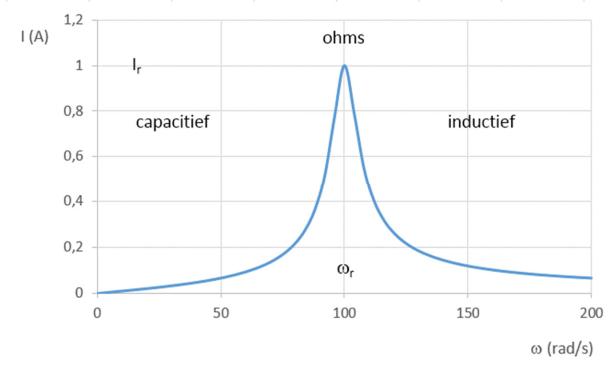
\includegraphics[width=0.5\textwidth]{resonatie.png}
        \caption{Resonantie in een RLC-seriekring. Bij de resonantiefrequentie $f_0$ zijn de inductieve en capacatieve reactanties gelijk, waardoor de totale impedantie minimaal is en de stroom maximaal.}
        \label{fig:resonatie.png}
\end{figure}
\FloatBarrier


\section{Hoofdstuk 3: Elektrische netwerken}
Er zijn geen nieuwe formules in dit hoofdstuk.
Het wilt vooral tonen dat netwerk analyse (zie elektrische netwerken) ook kan toegepast worden op 
AC netwerken.

\frm{Belastingen in serie}{Z_{totaal} = Z_1 + Z_2 + ... + Z_n}{Met $Z_{totaal}$ de totale impedantie in Ohm en $Z_1, Z_2, ..., Z_n$ de individuele impedanties in Ohm.}

\frm{Belastingen in parallel}{\frac{1}{Z_{totaal}} = \frac{1}{Z_1} + \frac{1}{Z_2} + ... + \frac{1}{Z_n}}{Met $Z_{totaal}$ de totale impedantie in Ohm en $Z_1, Z_2, ..., Z_n$ de individuele impedanties in Ohm.}

In parallel:
\[Z_{totaal} = \frac{1}{\frac{1}{Z_1} + \frac{1}{Z_2}} = \frac{Z_1 Z_2}{Z_1 + Z_2}\]

Zorg dat je niet verward geraakt omdat capaciteiten en inductanties imaginaire impedanties zijn.
Je gebruikt gewoon dezelfde regels als bij DC netwerken.


\begin{examenbox}
Zorg dat je de slides van dit hoofdstuk goed bekijkt.
Thevenin en Norton komen hier terug aan bod.
Als je vorig jaar elektrische netwerken goed begreep zou dit ook moeten lukkken.
\end{examenbox}

\section{Hoofdstuk 4: Driefasige wisselstromen}

Stel je drie bronnen voor die elk 120 graden verschil hebben 
met elkaar.

\[V_1 = V_m \sin(\omega t)\]
\[V_2 = V_m \sin(\omega t + 120^\circ)\]
\[V_3 = V_m \sin(\omega t - 120^\circ)\]

$V_m is gelijk voor alle drie de fasen.$

\begin{figure}[ht]
      \centering
        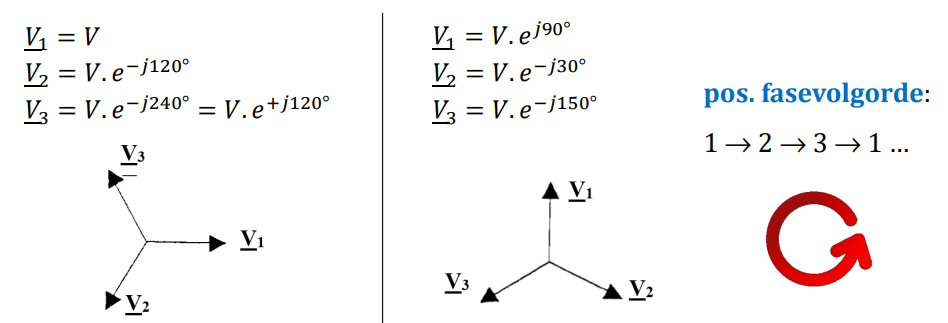
\includegraphics[width=0.8\textwidth]{3-fase.png}
        \caption{Driefasige spanningsysteem die de drie fasen toont met een faseverschil van 120 graden tussen elke fase.}
        \label{fig:3-fase.png}
\end{figure}

\begin{figure}[ht]
      \centering
        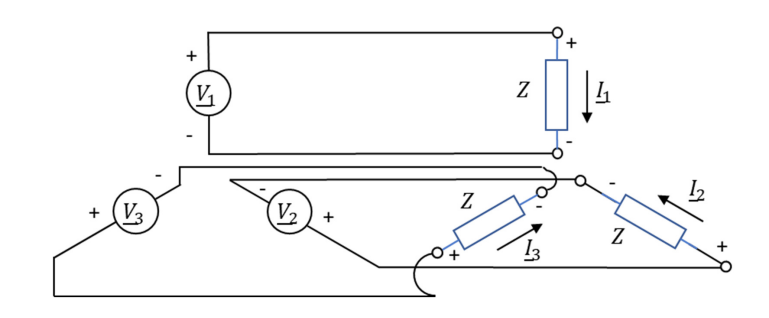
\includegraphics[width=0.45\textwidth]{circuit3-fase.png}
        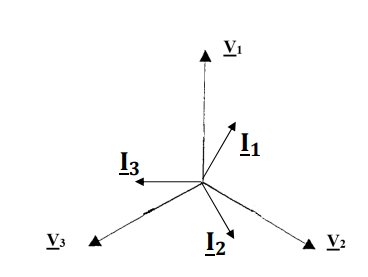
\includegraphics[width=0.45\textwidth]{fasors3fase.png}
        \caption{Driefasig circuit met drie fasen die elk 120 graden uit fase zijn.}
        \label{fig:circuit3-fase.png}
\end{figure}
\FloatBarrier

De stromen gaan voor of achter lopen afhankelijk van de belasting.
In de figuur loopt het achter dus de stroom is lagging -> impedantie is inductief L.
\newline

Hoe kunnen we nu de hoeveelheid draden in dit systeem verminderen?
We kunnen een ster- of driehoekconfiguratie gebruiken.

\subsection{Sterconfiguratie}

\begin{figure}[ht]
      \centering
        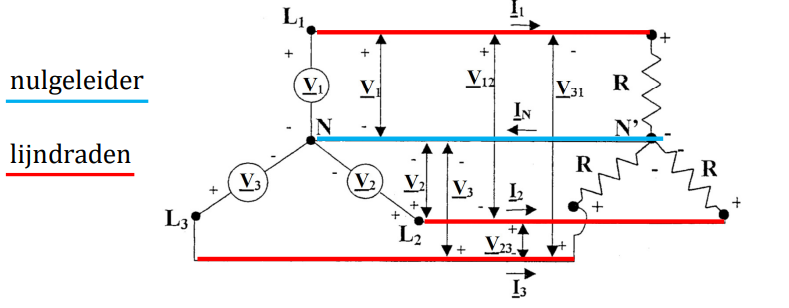
\includegraphics[width=1\textwidth]{ster.png}
        \caption{Sterconfiguratie van een driefasig systeem waarbij elke fase verbonden is met een gemeenschappelijk nulpunt
        \textbf{De nulgeleider}.}
        \label{fig:ster.png}
\end{figure}

\begin{description}
    \item[Lijnspanning]: De spanningen tussen de lijnen onderling $V_L$.
    \item[fasespanning]: De spanning tegenover de nulgeleider $V_f$.
    \item[Lijnstroom]: De stroom door de lijndraden $I_L$. 
    \item[Fasestroom]: De stromen geleverd door de bronnen $I_f$
\end{description}

We nemen aan dat de belasting gelijk is voor elke fase.

\subsubsection{Relatie tussen stromen en spanningen}
Omdat de belasting gelijk is voor elke fase zijn de fasestromen(de stromen door de weerstanden)
en de lijnspannignen (de spanningen tegenover de nulgeleider) ook gelijk.

\[\vec{I_{L1}} = \vec{I_{f1}}\]
\[\vec{I_{L2}} = \vec{I_{F2}}\]
\[\vec{I_{L3}} = \vec{I_{F3}}\]

\[I_N = I_{f1} + I_{f2} + I_{f3}\]
Bij evenwichte belastingen is de som van de fasestromen nul dus:
\[\vec{I_N} = 0 = I_{f1}+ I_{f2} + I_{f3}\]

\begin{minipage}{0.45\textwidth}
Deze figuur lijkt eerst verrarrend maar het geeft ons de 
relaties tussen de spanningen.
Dit zijn de fasors van de bronspanningen met de lijnspanningen.
We weten uit het schema dat:
\[V_{12} = V_{1} - V_{2}\]
\[V_{23} = V_{2} - V_{3}\]
\[V_{31} = V_{3} - V_{1}\]
\newline
MN is de helft van de lijnspanning dus:
\[2MN = V_{L1}\]
met $$MN = V_{f1}\cdot \cos(30^\circ)$$
\[V_{L1} = 2 V_{f1} \cdot \cos(30^\circ) = \sqrt{3} V_{f1}\]
\newline
De 30 graden komt door het verschil tussen fasespanning $V_{f1}<90^\circ$ en $V_{f2}<-30^\circ$. 
met $V_{f1}$-$V_{f2}$ =>120°. $V_L$ is dus 120° gedraait.
\end{minipage}
\begin{minipage}{0.45\textwidth}
\centering
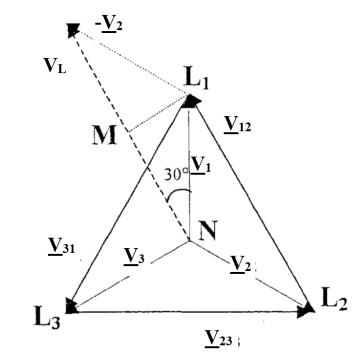
\includegraphics[width=0.5\textwidth]{fasors.png}
\end{minipage}


Deze relaties gelden alleen voor \belangrijk{evenwichtige belastingen}.
\frm{Relatie lijn- en fasespanning \& stromen in sterconfiguratie}
{\vec{V_L} = \sqrt{3} \cdot \vec{V_f} \quad , \quad \vec{I_L} = \vec{I_f}}
{Met $\vec{V_L}$ de lijnspanning in Volt, $\vec{V_f}$ de fasespanning in Volt, 
$\vec{I_L}$ de lijnstroom in Ampère en $\vec{I_f}$ de fasestroom in Ampère.}

Voorbeeld: Je hebt een 3-fase stersysteem met een fasespanning van $230 V$.
Wat is de lijnspanning?
\[\vec{V_L} = \sqrt{3} \cdot \vec{V_f} = \sqrt{3} \cdot 230 V = 398.37 V\]
\newline
Nog een voorbeeld: Je hebt een 3-fase stersysteem met een lijnstroom van $10 A$.
Wat is de fasestroom?
\[\vec{I_L} = \vec{I_f} = 10 A\]
\newline
Nog een laatse: Je hebt een 3-fase stersysteem met een lijnspanning van $400 V$. Je hebt een fasestroom van $5 A<30^\circ$.
Wat is de fasespanning? Wat is de lijnstroom? De impedantie van elke fase?
\[\vec{V_L} = 400 V\]
\[\vec{V_f} = \frac{\vec{V_L}}{\sqrt{3}} = \frac{400 V}{\sqrt{3}} = 230.94 V\]
\[\vec{I_L} = \vec{I_f} = 5 A < 30^\circ\]
\[\vec{Z_f} = \frac{\vec{V_f}}{\vec{I_f}} = \frac{230.94 V}{5 A < 30^\circ} = 46.19 \angle -30^\circ \Omega = 40 + j23.09 \Omega\]
\newline

\subsection{Driehoekconfiguratie}
Bij een driehoekconfiguratie zijn de belastingen en bronnen verbonden in een driehoek.

Snelle herhaling van de definities:
\begin{itemize}
  \item Lijnspanning de spanning om de lijnen onderling $V_L$.
  \item Fasespanning de spanning over elke belasting $V_f$.
  \item Lijnstroom de stroom door de lijndraden $I_L$.
  \item Fasestroom de stromen geleverd door de bronnen $I_f$.
\end{itemize}

\begin{figure}[ht]
  \centering
    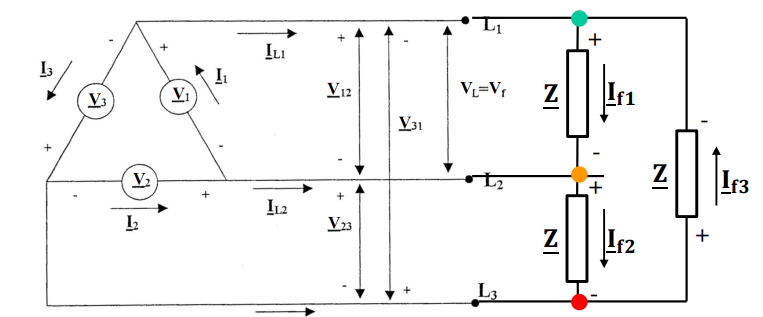
\includegraphics[width=1\textwidth]{driehoek 3fasesyteem.png}
      \caption{}
        \label{fig:driehoek 3fasesyteem.png}
      \end{figure}

      Omdat de bronnen gelijk aan elkaar zijn verbonden is het 
      verschil tussen de lijnspanningen en fasespanningen nul.
      \[\vec{V_{L1}} = \vec{V_{f1}}\]
      \[\vec{V_{L2}} = \vec{V_{f2}}\]
      \[\vec{V_{L3}} = \vec{V_{f3}}\]

      Als de belastingen gelijk zijn, zijn er geen terug stromingen door de bronnen.

      Als kirckoff toepassen op de knooppunten krijgen we:
      \[\vec{I_{L1}} = \vec{I_{f1}} - \vec{I_{f3}}\]
      \[\vec{I_{L2}} = \vec{I_{f2}} - \vec{I_{f1}}\]
      \[\vec{I_{L3}} = \vec{I_{f3}} - \vec{I_{f2}}\]

      Analoog aan de sterconfiguratie maar nu voor de stromen:

Deze relaties gelden alleen voor \belangrijk{evenwichtige belastingen}.

\frm{Relatie lijn- en fasestromen \& spanningen in driehoekconfiguratie}
{\vec{I_L} = \sqrt{3} \cdot \vec{I_f} \quad , \quad \vec{V_L} = \vec{V_f}}
{Met $\vec{I_L}$ de lijnstroom in Ampère, $\vec{I_f}$ de fasestroom in Ampère, 
$\vec{V_L}$ de lijnspanning in Volt en $\vec{V_f}$ de fasespanning in Volt.}

\begin{figure}[ht]
  \centering
    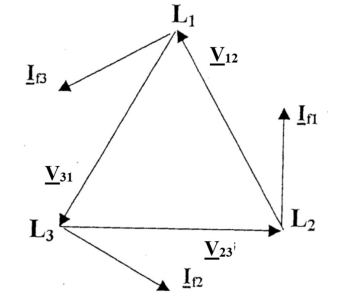
\includegraphics[width=0.4\textwidth]{fasorsindriehoek.png}
    
\includegraphics[width=0.4\textwidth]{image4.png}
    \caption{Driehoekconfiguratie fasordiagram van de lijn en fasespanningen en de }
    \label{fig:fasorsindriehoek.png}
\end{figure}

\subsection{3-fase vermogen}

In een 3-fase systeem is het totale vermogen de som van de vermogens in elke fase.
\newline
	\textbf{Belangrijk:} in de vermogensformules is $\phi$ de fasehoek \textbf{tussen spanning en stroom van de belasting} (arbeidsfactorhoek / impedantiehoek). Dit is \textbf{niet} het $120^\circ$ faseverschil tussen de drie bronspanningen.
\frm{Totaal vermogen in 3-fase systeem}{P_{totaal} = \sum_{n=1}^{3} P_{fase} = 3 \cdot P_{fase}}
{Met $P_{totaal}$ het totale actieve vermogen in Watt en $P_{fase}$ het actieve vermogen per fase in Watt.}


met gelijke belastingen in elke fase:
\[P_{totaal} = 3 \cdot P_{fase}\]
Met het vermogen per fase:
\frm{Vermogen per fase in 3-fase systeem}{P_{fase} =3 V_f \cdot I_f \cdot \cos \phi}
{Met $P_{fase}$ het actieve vermogen per fase in Watt, $V_f$ de fasespanning in Volt, 
$I_f$ de fasestroom in Ampère en $\phi$ de fasehoek tussen $V_f$ en $I_f$ (dus tussen spanning en stroom van de belasting) in radialen.}

Als we de relaties tussen lijn- en fasespanningen voor ster- en driehoekconfiguraties invullen krijgen we:

\begin{figure}[ht]
  \centering
    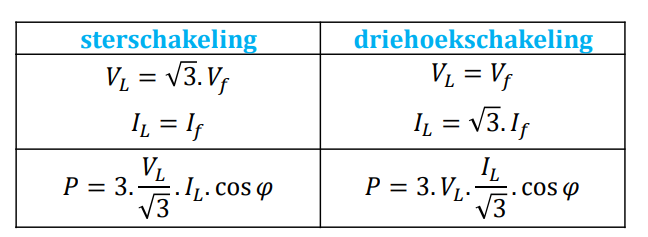
\includegraphics[width=0.8\textwidth]{totaalvermogen.png}
  \caption{Totaal vermogen in een 3-fase systeem voor zowel ster- als driehoekconfiguraties. In beide gevallen is het totale actieve vermogen $P_{totaal} = \sqrt{3} V_L I_L \cos \phi$, waarbij $\phi$ de fasehoek is tussen spanning en stroom van de belasting (arbeidsfactorhoek), niet het $120^\circ$ faseverschil tussen de fasen.}
  \label{fig:totaalvermogen.png}
\end{figure}

\frm{Totaal vermogen in 3-fase systeem}{P_{totaal} = \sqrt{3} V_L \cdot I_L \cdot \cos \phi}
{Met $P_{totaal}$ het totale actieve vermogen in Watt, $V_L$ de lijnspanning in Volt, 
$I_L$ de lijnstroom in Ampère en $\phi$ de fasehoek tussen spanning en stroom van de belasting (arbeidsfactorhoek) in radialen.}


\subsection{2-wattmethode}
Als we het vermogen willen meten maar de belastingen zijn niet gelijk kunnen we de 2-wattmethode gebruiken.
Bij gelijke belastigen is het simpelweg $P_{totaal} = 3 \cdot P$.

Als de belastingen niet gelijk zijn kunnen we de 2-wattmethode gebruiken.

\begin{figure}[ht]
    \centering
      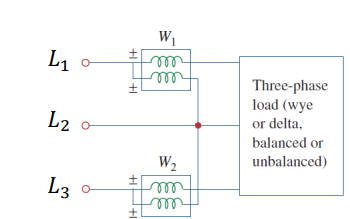
\includegraphics[width=0.6\textwidth]{2-wattmethode.png}
      \caption{2-wattmethode voor het meten van het totale actieve vermogen in een 3-fase systeem met ongelijke belastingen. Door twee wattmeters aan te sluiten op specifieke lijnen, kunnen we het totale vermogen berekenen als $P_{totaal} = P_1 + P_2$.}
      \label{fig:2-wattmethode.png}
\end{figure}
\FloatBarrier

\frm{2-wattmethode}{P_{totaal} = P_1 + P_2}{Met $P_{totaal}$ het totale actieve vermogen in Watt, $P_1$ het vermogen gemeten door wattmeter 1 in Watt en $P_2$ het vermogen gemeten door wattmeter 2 in Watt.}

De wattmaters meten de fasestroom en de lijnspanning.

\[P_1 = V_{12} \cdot I_{f1} \cdot \cos (30^\circ + \phi_1) = V_L \cdot I_L \cdot \cos (30^\circ + \phi_1)\]
\[V_{23} = -V_{32}\]
$V_{32}$ ijlt achter op $V_{3}$ met 30 graden
\[P_2 = V_{32} \cdot I_{f3} \cdot \cos (-30^\circ + \phi_3) = V_L \cdot I_L \cdot \cos (-30^\circ + \phi_3)\]

\begin{figure}[ht]
    \centering
      
\includegraphics[width=0.45\textwidth]{image5.png}
      
\includegraphics[width=0.45\textwidth]{image6.png}
      \caption{}
      \label{fig:image5.png}
\end{figure}

\frm{Totale vermogen in 2-wattmethode}{P_{totaal} = 3V_f \cdot I_f \cos{\theta}  =\sqrt{3} V_L \cdot I_L \cos{\theta}
}{Met $P_{totaal}$ het totale actieve vermogen in Watt, $V_L$ de lijnspanning in Volt, 
$I_f$ de fasestroom in Ampère, $V_f$ de fasespanning in Volt, 
$I_L$ de lijnstroom in Ampère en $\theta$ de hoek tussen de spanning en stroom}

Het reactief vermogen kan je ook berekenen met de 2-wattmethode.
\[Q_{totaal} = P1 - P2\]
\[Q_{totaal} = V_L \cdot I_L \cdot \cos(30^\circ + \phi_1) - V_L \cdot I_L \cdot \cos(-30^\circ + \phi_3)\]
\[Q_{totaal} = V_L \cdot I_L [\cos(30^\circ + \phi_1) - \cos(-30^\circ + \phi_3)]\] 
\[Q_{totaal} = \sqrt{3} V_L \cdot I_L \sin{\theta}\]

\frm{reactief vermogen in 2-wattmethode}{Q_{totaal} = \sqrt{3}(P_2 - P_1 = \sqrt{3} V_L \cdot I_L \sin{\theta})
}{Met $Q_{totaal}$ het totale reactieve vermogen in Volt-Ampère reactief 
(VAR), $P_1$ het vermogen gemeten door wattmeter 1 in Watt en $P_2$ het vermogen gemeten door wattmeter 2 in Watt.}


\frm{fasehoek}{\theta = tan^{-1}\left(\frac{Q_{totaal}}{P_{totaal}}\right)= tan^{-1}\left(\frac{\sqrt{3}(P_2 - P_1)}{P_1 + P_2}\right)
}
{Met $\theta$ de gemiddelde fasehoek tussen spanning en stroom van de belastingen, 
$Q_{totaal}$ het totale reactieve vermogen in Volt-Ampère reactief (VAR) en $P_{totaal}$ het totale actieve vermogen in Watt.}

Het schijnbaar vermogen wordt berekend als volgt:

$S_{totaal} = P_{totaal} + j Q_{totaal}$

\frm{schijnbaar vermogen in 2-wattmethode}{S = 3 V_f \cdot I_f = 3\frac{V_L^2}{Z} = 3 I_L^2 Z}
{Met $S$ het schijnbaar vermogen in Volt-Ampère (VA), $V_L$ de lijnspanning in Volt, 
$I_f$ de fasestroom in Ampère, $I_L$ de lijnstroom in Ampère en $Z$ de impedantie van de belasting in $\Omega$ .}


\begin{figure}[ht]
  \centering
    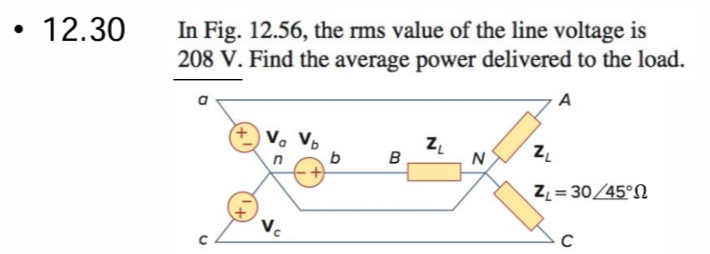
\includegraphics[width=0.8\textwidth]{vboefening 3fase.png}
    \caption{Ster configuratie met gelijk belastingen.}
      \label{fig:vboefening 3fase.png}
    \end{figure}
    \FloatBarrier

    \[V_l = 208 V\]
    \[V_f = \frac{V_l}{\sqrt{3}} = \frac{208 V}{\sqrt{3}} = 120.1 V\]
    \[I_f = \frac{V_f}{Z_L} = \frac{120.1 V}{30<45^\circ \Omega }\]
    rekenmachine in r<theta modus
    \[I_f = 4.0 < -45^\circ A\]
    \[P = 3 V_f I_f \cos \phi = 3 \cdot 120.1 V \cdot 4.0 A \cdot \cos 45^\circ = 1021.6 W\]
    \[Q = 3 V_f I_f \sin \phi = 3 \cdot 120.1 V \cdot 4.0 A \cdot \sin 45^\circ = 1021.6 VAR\]
    \[S = P + jQ = 1021.6 W + j 1021.6 VAR = 1445.6 VA\]



\section{Conclusie}
Dit document bevat meeste relevante formules maar
je moet oefeningen maken om ze goed te begrijpen.

\begin{center}

	\itshape\Huge

	Veel succes met de examens!

	\par\vspace{1cm}

	\normalfont\Large

	--- Ruben Ryckaert

\end{center}







\end{document}
